\chapter{Uitwerken prototype ---GEKOZEN FRAMEWORK---}
\label{ch:prototype}

Hierin zal een uitleg komen over de uitwerking van het gekozen prototype en de manier waarop ik gewerkt hebt. De IDE waarin ik gewerkt zal hebben zal hier ook kort besproken worden, vooral de ondersteuning voor het framework waarin ik werk zal hier een grote rol spelen.
De gemaakte keuzes i.v.m. met de ervaring zal hier ook besproken worden.
\begin{figure}
    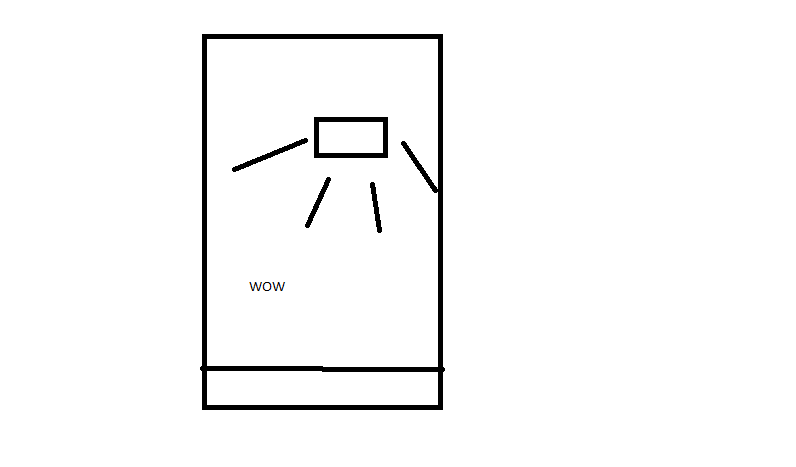
\includegraphics[width=\textwidth]{img/wow}\caption{Het herkennen van een afbeelding doet iets}\label{fig:imgreg1}
\end{figure}